

\section{Errors}
In this section, we will present three types of errors that we implemented in the simulation: path jitter, dephasing and data qubit displacement. The path jitter is implemented in the calculation of the Hamiltonian for each new spatial point, whereas the dephasing is introduced through a Lindblad operator. Finally, data qubit displacement is simulated by a random offset for each of the four data qubits. In connection to qubit displacement, we will also review a technique called twirling and show how it affects our simulations. Let us begin by introducing a path jitter into the simulation. 


\subsection{Error benchmarking}
There are two different ways to quantify error, and we shall here quickly review them as they will be used extensively in the following sections. 

The first way to quantify error is to look at the phase $\phi$ accumulated by the probe qubit through the interaction with the data qubits. In \cite{the paper}, the phase jitter is defined as $\phi + \delta$, where $\delta$ is a small deviation from $\frac{\pi}{2}$, which is the ideal phase accumulated through one quarter of the cycle. In the paper, it was found that a phase jitter of $4.4 \%$ did not have a substantial impact on the fault-tolerance threshold. We will therefore attempt to compare the phase error in our simulation with this value whenever possible. It should be noted, however, that the data we have access to usually concerns the entire run. We will therefore compare the phase error with $2\pi$ or $\pi$. We have made the assumption that the phase error stacks, such that the percentage is preserved. 


%\clearpage
\subsection{Path Jitter}\label{sec:jitter}
The fist error that we shall introduce is jitter present in the orbit performed by the probe qubit. The precision provided by modern MEMS control structures is about 1 nm \cite{MEMS precision} and is due to improve in the near future, but that does ont leave it impervious to noise. At first, we attempted to simulate random jumpts in the trajectory, but discontinuities in the path led to large derivative terms which in turn caused the simulation to fail. Instead, we superposed a sinusoidal motion onto the trajectory path. To add a random element, we varied the phase with which the run start while selecting the amplitude of the motion to represent the uncertainty in precision. The results can be found in Figure \ref{fig:pathjitter}, where we note that an uncertainty of about 2 nm is sufficient for staying below the phase error threshold of $4.4 \%$. Here, we are not comparing the phase jitter with the measurement probability since the probe qubit is not undergoing dephasing due to this interaction. It is sufficient to look at jitter in the $y$-direction instead of both the $x$ and $y$ direction, since the phase error is symmetric between them. 



\begin{figure}[h]
  \centering
    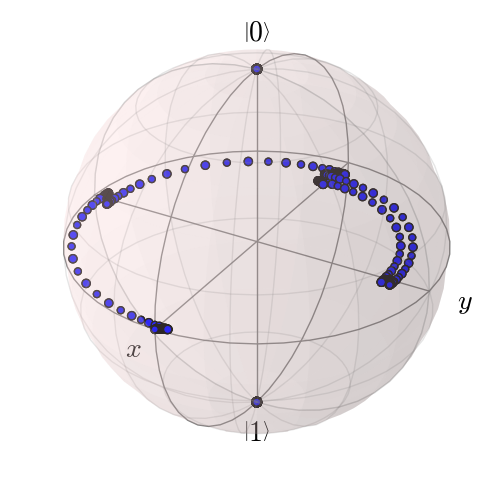
\includegraphics[width=0.5\textwidth]{../Figures/Circ_orbit_odd_100_dephasing.png}
      \caption{ }
      \label{fig:pathjitter}
\end{figure}


From the graph it also becomes clear that jitter in the $z$-direction has the greatest influence. This is due to the $\frac{1}{r^3}$  term in the Hamiltonian which favours the influence of the $z$-direction. 





\subsection{Dephasing}
Next, we looked at the influence of dephasing on the measurement probabilities. In order to simulate dephasing, which is the gradual reduction of the Bloch vector in the $x$-direction, we introduced a Lindblad operator into the master equation. The operator is given by 
\beq
L  = \sqrt{\Gamma} \sigma_z,
\eeq
where $\Gamma$ is the dephasing parameter, which can also be written as $1/\tau$ where $\tau$ is the dephasing time. Since dephasing does not affect the phase accumulated over the four runs, we do not end up with a phase error, except when our state completely decoheres and the phase information becomes unavailable. Therefore, the only accurate measure of the error becomes the probability of correctly measuring the stabiliser in either the $\ket{+}$ (even parity) or $\ket{-}$ (odd parity). We ran simulations for both the abrupt and circular orbit using the $T_2$ and $T_2^*$ values in Table \ref{tab:spinspecies}. The results can be found in Figure \ref{fig:dephasing}, where each number refers to an entry in the table. 

We see that the clock transition in Bismuth does exceptionally well, but that many spin species decohere before the run is completed. This is especially notable in the case for the circular orbit, which takes approximately $10$ times longer than the abrupt orbit. It should be noted however that data for the spin species which decohere completely is for the $T_2^*$ time measured without the aid of Hahn echoes \cite{hahn} or dynamic decoupling \cite{something}. Implementing these additional techniques would significantly improve the dephasing time for many of the proposed spin species. 

As we discuss in more detail in Section \ref{sec:Outlook}, the impact of dephasing could be decreased by lowering the time needed for the probe qubit to complete one orbit around the data qubits. This would require lowering the distance $d$ between the probe qubits and the data qubits as to increase the interaction strength between them. 


\begin{figure}[H]
	\subfloat[]{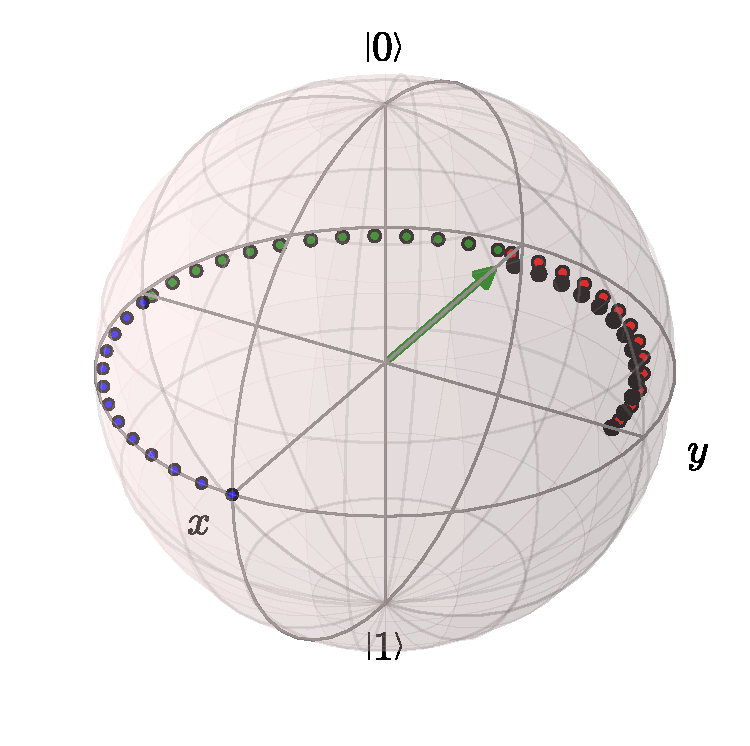
\includegraphics[width=0.49\linewidth]{../Figures/abrupt-deph} \label{FIG:abr-deph}}
	\subfloat[]{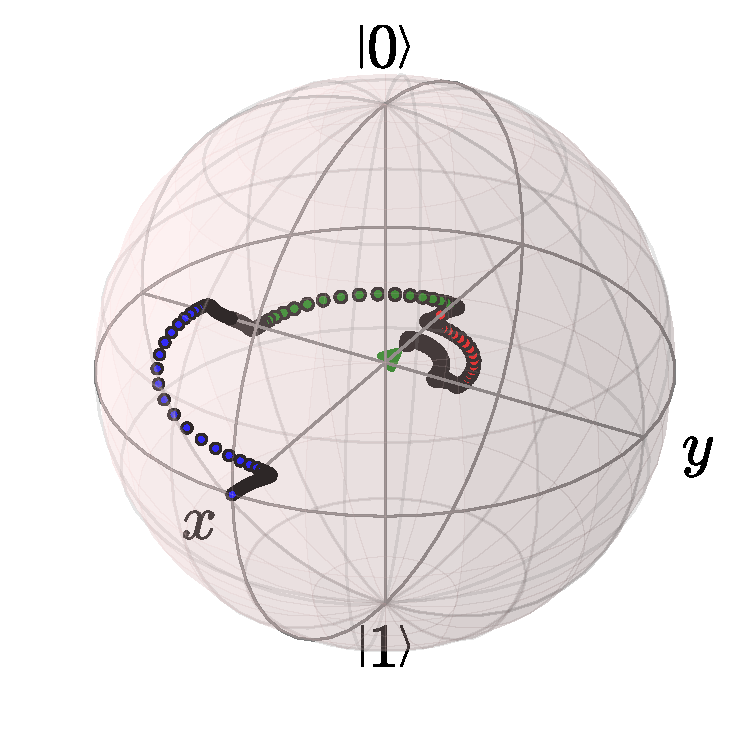
\includegraphics[width=0.49\linewidth]{../Figures/circ-deph} \label{FIG:circ-deph}}
	\caption[oddeven]{}
	\label{FIG:deph}
\end{figure}


\begin{figure}[h]
  \centering
    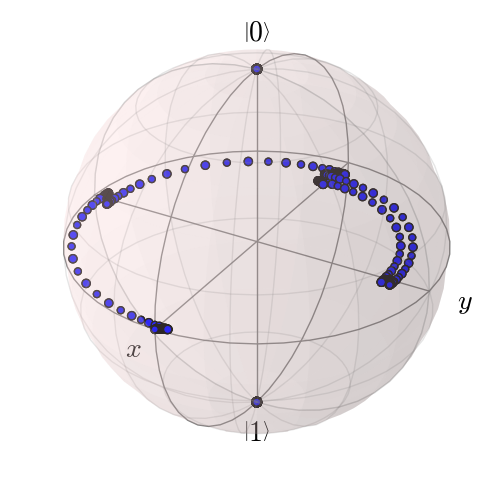
\includegraphics[width=0.5\textwidth]{../Figures/Circ_orbit_odd_100_dephasing.png}
      \caption{The states of the probe and data qubits plotted in the Bloch sphere with a dephasing parameter of 100, which translates to a dephasing time of 10 ms. The phase of the probe qubit is not affected since no relaxation or excitation is taking place. The effect can however be seen in the probability of measuring the probe qubit in the $\ket{+}$ or $\ket{-}$ state. For complete dephasing, the probe qubit will become the maximally mixed state and the measurement outcomes are completely random. The states of the probe and data qubits plotted in the Bloch sphere with a dephasing parameter of 100, which translates to a dephasing time of 10 ms.}
      \label{fig:BlochsphereDephasing}
      
\end{figure}


\begin{figure}[!h]
  \centering
    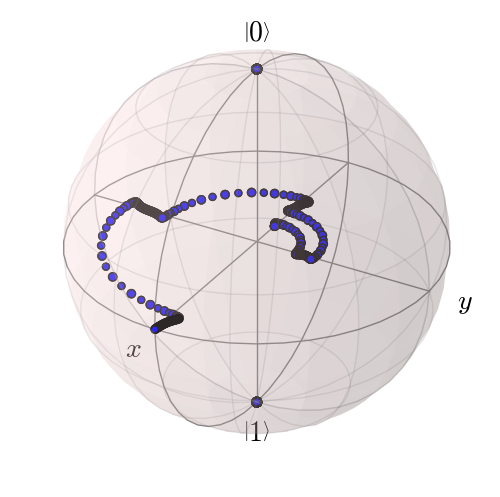
\includegraphics[width=0.5\textwidth]{../Figures/Circ_orbit_odd_500_dephasing.png}
      \caption{The states of the probe and data qubits plotted in the Bloch sphere with a dephasing parameter of 500, which translates to a dephasing time of 2 ms. The strong dephasing causes the probe qubit state to drift quickly towards the maximally mixed state. }
      \label{fig:BlochsphereDephasing2}
\end{figure}




\begin{figure*}[h]
	\centering
	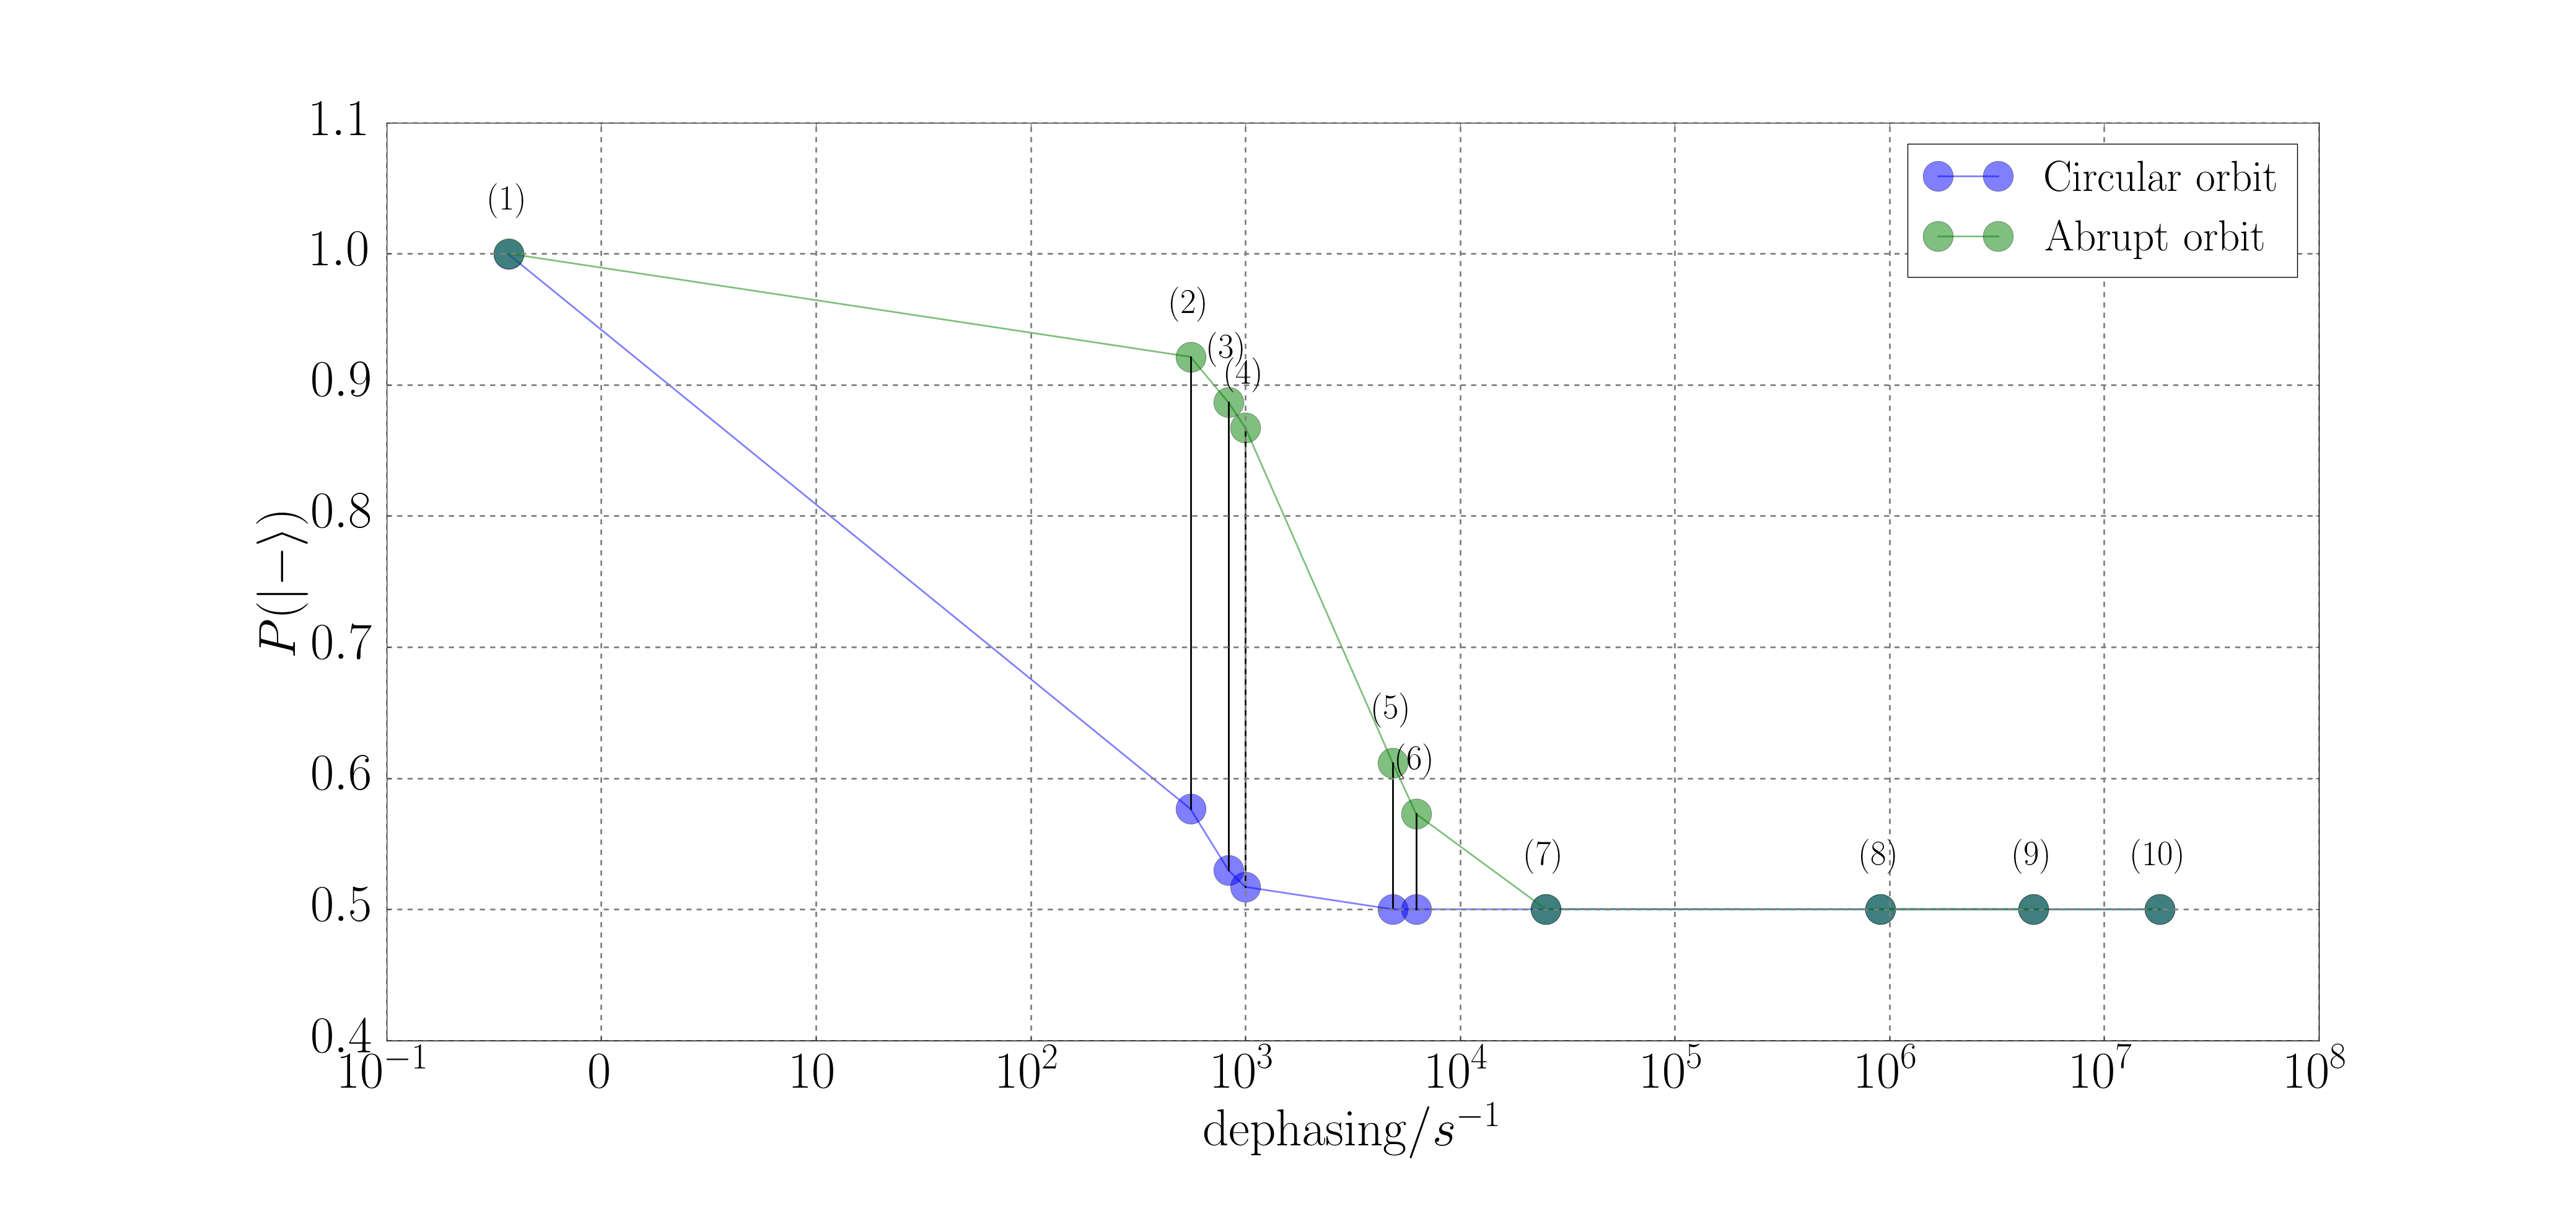
\includegraphics[width=\textwidth]{../Figures/dephasing_plot.png}
		\caption{A graph showing the relationship between the dephasing parameter $\Gamma$ and the probability $P(\ket{-})$ of measuring the probe qubit in the $\ket{-}$ state. In this simulation, one of the data qubits have undergone a bit-flip error. As the dephasing parameter increases, the probe qubit moves towards the maximally mixed state and the probability of measuring $\ket{-}$ goes towards 0.5.}
		\label{fig:phaseplot}
\end{figure*}





